\chapter{Sicherheitsdienste}\label{Sicherheitsdienste}

Nachdem wir in den vorherigen Kapiteln\dots
Es folgt eine Untersuchung wie konkret die Sicherheitanforderungen implementiert werden können.
TODO (Benita)

\section{Vertraulichkeit}
\section{Authentifizierung}

Authentifizierung sogrt dafür, dass ein Benutzer gegenüber einem System verifiziert werden kann.
Der Begriff der Authentifizierung wird oft synonym mit den Begriffen Authentisierung und Autorisierung verwendet. 
Die Authentifizierung lässt sich in weitere Bestandteile untergliedern. Der erste Bestandteil ist die Authentisierung, 
wobei der Benutzer gegenüber dem System eine Identität vorgibt, die von diesem bestätigt werden soll. 
Auf die Authentisierung folgt anschließend die Authentifizierung. Bei dem Authentifizierungsvorgang werden die vom Nutzer 
eingegebenen Daten, also seine angegebene Identität, überprüft. Ist die Überprüfung abgeschlossen folgt die 
Autorisierung. Die Autorisierung ist für die Zuteilung der Zugriffsrechte verantwortlich. 
Durch den Prozess der Authentifizierung wird eine Identität an ein Subjekt/ Entität gebunden. 
Das Binden der Identität berechtigt den Benutzer bestimmte Dienste in Anspruch nehmen zu können. 
\newline
Es gibt verschiedene Arten wie eine Authentifizierung durchgeführt werden kann:
\begin{figure}[H]
    \centering
    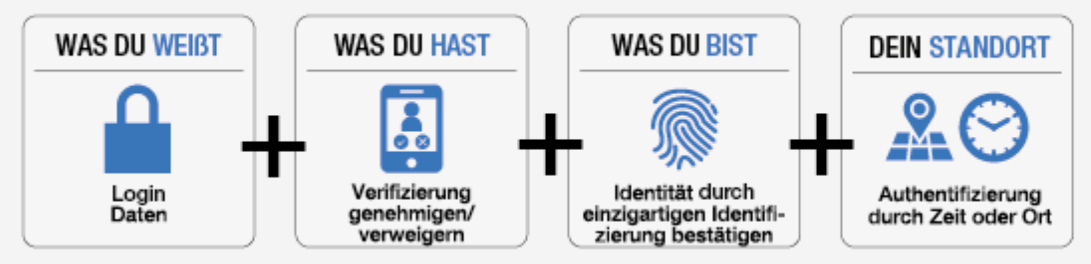
\includegraphics[width=\textwidth]{images/authent_pos1.png}
    \caption[Authentifizierungsarten]{Authentifizierungsarten} 
    \label{Authentifizierungsarten}
\end{figure} 
Im Zusammenhang mit der Ausarbeitung wird immer wieder die Methode der Authentifizierung durch Wissen, 
also Login mittels Benutzername und Password, aufgegriffen. 


\section{Integrität}
\section{Nicht-Anfechtbarkeit}
\section{Zugriffssteuerung/Autorisierung}
\section{Verfügbarkeit}